\documentclass[a4paper,11pt]{article}
\usepackage{graphicx}
\usepackage[T1]{fontenc} % codifica dei font in uscita
\usepackage[utf8]{inputenc} % lettere accentate da tastiera
\usepackage[italian]{babel} % lingua principale del documento
\usepackage{url}
\usepackage [a4paper, top=2.5cm, bottom=2.5cm, left=1.5cm, right=1.5cm, bindingoffset=8mm] {geometry}

% inizio documento
             
\begin{document}

\begin{center}



\textsc{\Huge Esperienza V}\\[0.5cm]



\large
\title{ESPERIENZA IV}

Michele \textsc{Pedrotti}\\
Luigi \textsc{Bassini}\\
Nicola \textsc{Trevisson}\\


\end{center}
\vspace{0.1 cm}
\section{Scopo dell'esperienza}
 Lo scopo della nostra esperienza è la verifica della relazione empirica (legge di Lambert-Beer) che correla la quantità di luce assorbita da un mezzo alla natura chimica, alla concentrazione ed allo spessore del mezzo attraversato. La nostra esperienza, avendo a disposizione solamente il solfato di rame , si è svolta in due momenti: nella prima parte abbiamo variato la concentrazione della soluzione, mentre nella seconda abbiamo variato il cammino ottico (cioè lo spessore della soluzione attraversata).

\section{Misura dell'apertura numerica di una fibra ottica}
\subsection{Struttura di una fibra ottica}
La Fibra Ottica, che si presenta come un sottile filo di vetro, è costituita da un nucleo cilindrico (core) di un materiale trasparente, circondato da un mantello concentrico (cladding).La fibra è poi protetta esternamente da un rivestimento, in genere realizzato con materiale plastico, per la protezione dalle abrasioni.

 \begin{center} 
\begin{figure}[htpd]
\hspace{90 pt}
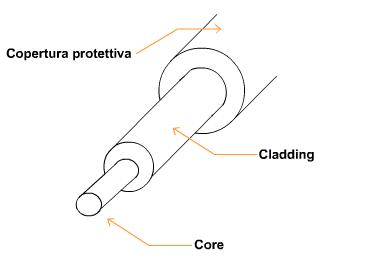
\includegraphics[scale=0.90]{fibre_ottiche.jpg}


\end{figure}
\end{center}

La fibra ottica funziona come una specie di specchio tubolare. La luce che entra nel core entro un certo angolo (angolo limite) si propaga mediante una serie di riflessioni sulla superficie di separazione fra i due materiali del core e del cladding.

\begin{center} 
\begin{figure}[htpd]
\hspace{90 pt}
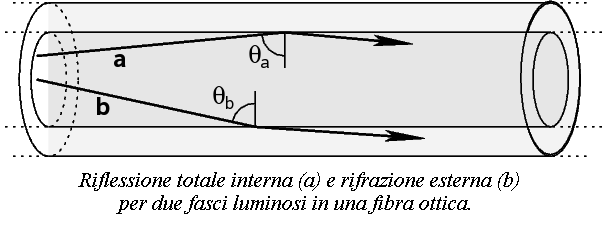
\includegraphics[scale=0.90]{Fibra_ottica2.png}


\end{figure}
\end{center}

Come mostrato in figura, se una radiazione elettromagnetica collide sulla superficie di separazione tra core e cladding con un angolo $\theta \textless \theta \ped{max}$, essa si propaga all'interno della fibra ottica. Al contrario, se essa 
collide sulla superficie di separazione con un angolo $\theta \textgreater \theta \ped{max}$, la radiazione viene rifratta all'esterno del core. 
\subsection{Calcolo dell'apertura numerica}
Il nostro apparato sperimentale consisteva in un laser nella lunghezza d'onda del rosso, una lente convergente, un carrello rotante, una fibra ottica e un fotodiodo. Il raggio del laser veniva concentrato mediante la lente convergente sulla superficie di uno dei capi della fibra ottica. Tale capo era montato su un carrello rotante dotato di goniometro. In questo modo, ruotando il carrello, era possibile variare l'inclinazione della superficie della fibra esposta ai raggi, e di conseguenza la percentuale dei fasci rifratti nel cladding. Per quantificare tale variazione all'altro capo della fibra era posto un fotodiodo, in grado di misurare la potenza della radiazione luminosa. \\
Il nostro obiettivo è quello di misurare l'apertura numerica NA, tramite la relazione: $$NA=n\ped{i}\cdot sin(\theta \ped{max}) $$  
Poichè l'esperimento è stato condotto a condizioni ambientali standard n$\ped{i}$=$n\ped{aria}$ $\simeq 1$. La conoscenza dell'apertura numerica è importante in quanto ci consente di conoscere il valore dell'angolo massimo affinchè le onde elettromagnetiche siano completamente riflesse all'interno del core. 
Per prima cosa è stato necessario trovare il valore massimo di potenza passante per la fibra. Questo è stato possibile variando l'angolo di inclinazione del carrello su cui era montata l'estremità della fibra esposta al laser. Durante questa fase abbiamo notato che l'angolo a cui corrisponde il valore massimo di intensità rilevata non era $ 0 $ (laser perpendicolare al capo della fibra) ma $ +1.25 $, con un valore di potenza misurato pari a 16$ \mu W $. L'angolazione differente da 0 può essere ricondotta a vari fattori, tra cui il non perfetto posizionamento della fibra o del laser sul loro supporto, o ancora il metoto con cui è stata tagliata la fibra. La sua superfice infatti può non essere regolare e presentare creste e scanalature dovute alle difficoltà pratiche di taglio che influenzano l'ingresso della luce all'interno del core.
Considerando questo valore di angolo come il nostro 0 abbiamo modificato l'angolo di incidenza dei fronti d'onda del laser sulla fibra.
Visto che le incognite erano due (l'angolo e l'intensità) abbiamo scelto di variare in maniera arbitraria la potenza rilevata dal fotodiodo. 
Di conseguenza la fibra è stata ruotata in modo da variare l'intensità di circa $ 1\mu W$, e si è quindi misurato l'angolo corrispondente. Una volta raggiunto il valore minimo di intensità luminosa, abbiamo riportato il carrello alla posizione di partenza, e annotato la potenza rilevata dal fotodiodo. Si è notato che l'intensità massima era variata sensibilmente, ma poichè questa variazione era inferiore al 5\%\ del valore iniziale abbiamo considerato i valori tra loro compatibili. La difficoltà di tale esperimento consisteva proprio in questo passaggio. La potenza del raggio luminoso prodotto dal laser non è infatti costante, ma dipende da numerosi fattori. Per esempio anche una minima vibrazione del tavolo di lavoro provocava una variazione della potenza rilevata dal fotodiodo. A questo punto abbiamo ruotato il carrello nella direzione opposta seguendo lo stesso procedimento. Abbiamo quindi riportato in un grafico i dati raccolti, inserendo sull'asse delle ordinate la potenza normalizzata in scala logaritmica,e sull'asse delle ascisse l'angolo corrispondente. Inoltre abbiamo rappresentato una retta corrispontente al 5\%\ della potenza massima. L'angolo corrispondente a questo valore sarà proprio $\theta \ped{max}$.  


\begin{center} 
\begin{figure}[htpd]
\hspace{-30 pt}
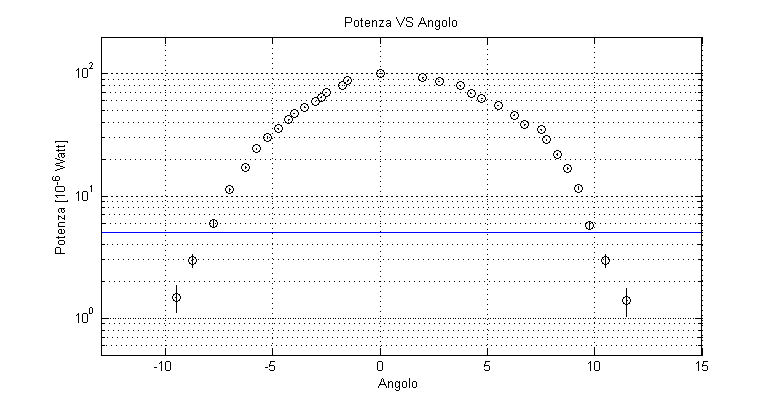
\includegraphics[scale=0.90]{Grafico_matlab.png}


\end{figure}
\end{center}
\vspace{5 cm}
Ci è dunque stato possibile calcolare l'apertura numerica tramite la relazione: $$NA=n\ped{i}\cdot sin(\theta \ped{max})= 0.60 \pm 0.05 $$  
Per ottenere questo valore abbiamo tenuto conto del valore ottenuto ruotando in entrambi i sensi il carrello, calcolando la media pesata tra i due valori.

\end{document}